\documentclass[a4paper]{jpconf}
\usepackage{graphicx}

% for code colouring
\usepackage{pgf,pgfarrows,pgfnodes,pgfautomata,pgfheaps,pgfshade}
\usepackage{amsmath,amssymb}
\usepackage[latin1]{inputenc}
\usepackage{colortbl}
\usepackage[procnames]{listings}
%%%%%%%%%%%%%%%%%%%%%

\usepackage{subfig}

%\usepackage[firstpage]{draftwatermark}
%\SetWatermarkText{draft-0.2}
%\SetWatermarkLightness{0.5}
%\SetWatermarkScale{8}

\begin{document}
\title{\texttt{docker} \& \texttt{HEP}:\\Containerization of applications for
development, distribution and preservation}

%\author{S\'ebastien Binet}

%\address{Laboratoire de l'Acc\'el\'erateur Lin\'eaire, Universit\'e
%  Paris-Sud XI, 91898, Orsay, FR}

\author{
  S. Binet, 
  B. Couturier\\
}

\ead{binet@cern.ch}

\begin{abstract}

HEP software stacks are not shallow.
Indeed, \texttt{HEP} experiments' software is usually many applications in one
(reconstruction, simulation, analysis, \ldots) and thus require many libraries --
developed in-house or by third parties -- to be properly compiled and installed.
Moreover, because of resource constraints, experiments' software is usually
installed, tested, validated and deployed on a very narrow set of platforms,
architectures, toolchains and operating systems.
As a consequence, bootstrapping a software environment on a developer machine or
deploying the software on production or user machines is usually perceived as
tedious and iterative work, especially when one wants the native performances of bare metal.

\texttt{Docker} containers provide an interesting avenue for packaging
applications and development environment, relying on the Linux kernel
capabilities for process isolation, adding \texttt{git}-like capabilities to the
filesystem layer and providing (close to) native CPU, memory and I/O performances.

\end{abstract}

\section{Introduction}

Development of High Energy and Nuclear Physics (\texttt{HENP}) software is
following more and more best practices devised in the industry.
These recipes help practitioners manage code versioning, ensure build
reproducibility and tame the unbridled growth of external
dependencies.
The tools developed in the software industry to cope (even at scale) with these
mundane issues have now percolated to some extent in \texttt{HENP} experiments.

Moreover, development and application isolation have been facilitated by the
increased usage of virtual machines, which also greatly helped portability.
However, even if production clusters are usually \texttt{Linux} systems running
\texttt{Linux} virtual machines, this portability comes at a price: resources overhead.

While virtual machines provide a machine-level virtualization environment,
containers provide an operating-system-level virtualization environment for
running multiple isolated operating-systems.
Containers seem to better match the main production use-case of typical
\texttt{HENP} clusters.
\texttt{LXC}~\cite{ref-lxc} and \texttt{OpenVZ}~\cite{ref-openvz} were the first to introduce containers into the
\texttt{Linux} ecosystem, but \texttt{Docker}~\cite{ref-docker} is the project that
really popularized and democratized them.

This paper explores the possible applications of \texttt{Docker} containers to
typical \texttt{HENP} workflows.
We first introduce in more details the \emph{modus operandi} of \texttt{Docker}
containers and then focus on the \texttt{hepsw/docks} containers which provide
containerized software stacks for -- among others -- the LHCb
Experiment~\cite{ref-lhcb} at CERN.
Then, we discuss various strategies experimented with to package software
(\emph{e.g.} \texttt{cvmfs}~\cite{ref-cvmfs}, \texttt{RPM}s, source-based) and how we applied
them to optimize provisioning speed and disk usage, leveraging the caching system of \texttt{Docker}.
Finally, we report on benchmarks comparing workloads on bare metal with regard
to \texttt{Docker} containers setups.

\section{A \texttt{Docker} primer}

\texttt{Docker} is an open source project to pack, ship and run any application
as a lightweight container.
 
% \begin{figure}[h]
% \begin{center}
% 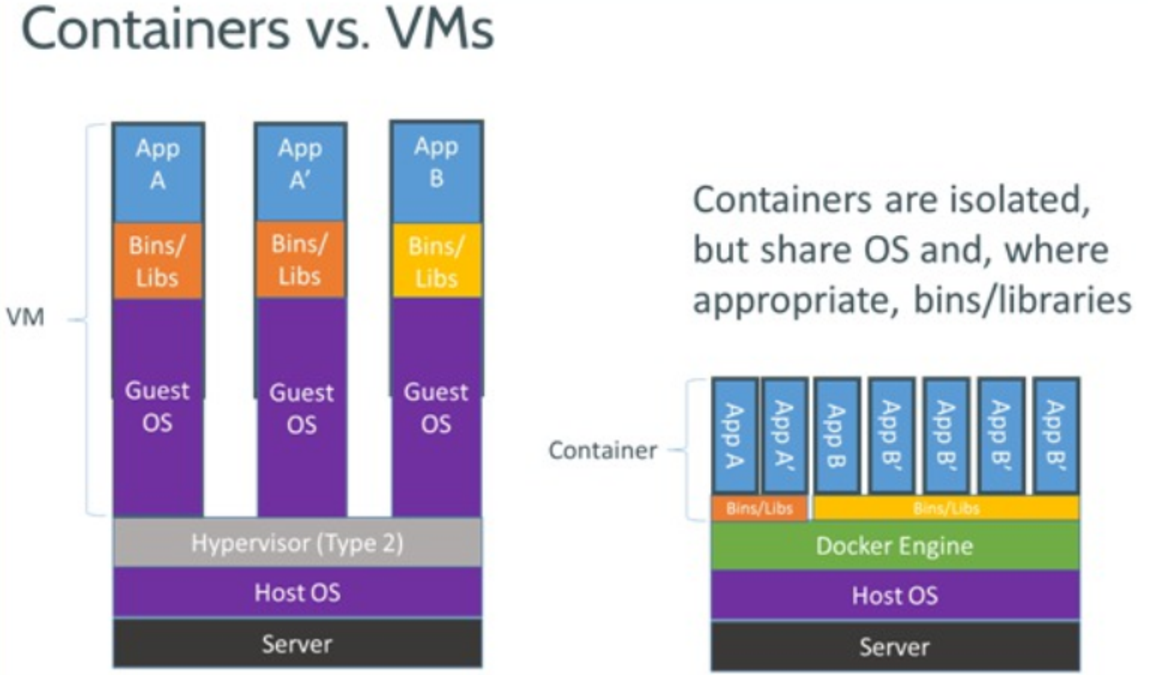
\includegraphics[width=0.8\linewidth]{figs/vm-lxc.pdf}
% \end{center}
% 	\caption{\label{fig-docker-overview}Comparaison of virtual machines (left)
% 	with containers (right).
% Rather than running a full OS on virtual hardware,
% container-based virtualization modifies an existing OS to provide
% extra isolation.}
% \end{figure}
 
\texttt{Docker} uses \texttt{Linux} namespaces,
\texttt{cgroups}~\cite{ref-cgroups} and unioning file systems to isolate
processes.
Container images are rather similar to virtual machine images, but share the
\texttt{Linux} kernel with the host machine.
This provides a much more lightweight setup and allows to provision container
images in seconds -- compared to minutes for virtual machines -- as well as to
run hundreds of such containers on a typical desktop machine.

Thanks to \texttt{cgroups}, containers can have their own network interface: in
layman's terms, containers can be seen as a super-\texttt{chroot}, with no
device emulation -- hence the almost bare metal performance.
\texttt{Docker} also provides a layered file system, building on unioning file
systems (\texttt{UnionFS}\cite{ref-unionfs}, \texttt{AUFS}~\cite{ref-aufs}) or
\texttt{device mapper}~\cite{ref-devicemapper} for
kernels without such modules.
Each layer of the file system is mounted on top of prior layers.
The first layer is the so-called \emph{base image}, holding an initial
collection of files and folders provided by a distribution (Ubuntu, RHEL,
Fedora, etc\ldots) which does not need to be the same as the host
distribution.
Each layer is read-only (only the top-layer is modifiable) and only stores on disk the \emph{delta} with regard to the previous
layer.
Individual layers are indexed by hashes \`a la \texttt{git} and can be shared
among images: this scheme enables very lightweight disk resources
requirements and thus, very fast disk provisioning performance.

\subsection{\texttt{Docker} images}
\texttt{Docker} images are created from a base container.
\texttt{Docker} ships a comprehensive set of \emph{official} base containers
(\texttt{ubuntu}, \texttt{centos}, etc\ldots) which can be downloaded locally
\emph{via} the \texttt{docker pull} command, as shown in
figure~\ref{fig-docker-pull}.

\begin{figure}[h]
\begin{lstlisting}[language=sh,
    basicstyle=\tiny,
    frame=trbl,
    numbers=left,
    showstringspaces=false,
    stringstyle=\ttfamily]
>> docker pull ubuntu
latest: Pulling from ubuntu
e9e06b06e14c: Pull complete 
a82efea989f9: Pull complete 
37bea4ee0c81: Pull complete 
07f8e8c5e660: Already exists 

Digest: sha256:8126991394342c2775a9ba4a843869112da8156037451fc424454db43c25d8b0
Status: Downloaded newer image for ubuntu:latest
\end{lstlisting}
\caption{\label{fig-docker-pull}\texttt{pull} retrieves a \texttt{docker} image
from the registry (also known as \texttt{docker hub}).}
\end{figure}

The list of local images can be queried using the \texttt{docker images}
command, as shown in figure~\ref{fig-docker-images}.

\begin{figure}[h]
	\begin{lstlisting}[language=sh,
		basicstyle=\tiny,
		frame=trbl,
		numbers=left,
		showstringspaces=false,
	stringstyle=\ttfamily]
>> docker images
REPOSITORY          TAG                 IMAGE ID            CREATED             VIRTUAL SIZE
ubuntu              latest              07f8e8c5e660        5 days ago          188.3 MB
centos              latest              fd44297e2ddb        2 weeks ago         215.7 MB
ubuntu              12.10               c5881f11ded9        10 months ago       172.1 MB
\end{lstlisting}
\caption{\label{fig-docker-images}\texttt{images} prints the list of local
images, retrieved from the registry or created locally.}
\end{figure}

Once an image is created or downloaded from the \texttt{Docker}
registry~\cite{ref-docker-hub},
it is possible to run an executable off that image, inside a container.
As shown in figure~\ref{fig-docker-run-hello}, it is also possible to specify an
explicit version (here $12.10$) for the image one wants to run.

\begin{figure}[h]
	\begin{lstlisting}[language=sh,
		basicstyle=\tiny,
		frame=trbl,
		numbers=left,
		showstringspaces=false,
	stringstyle=\ttfamily]
>> docker run ubuntu:12.10 echo "hello world"
hello world
\end{lstlisting}
\caption{\label{fig-docker-run-hello}\texttt{docker run} runs an executable
inside a container.
Here, the command \texttt{echo} is run on top of the base image \texttt{ubuntu},
explicitly using the version $12.10$ of that image.}
\end{figure}

It is also possible to run containers in detached mode, the typical use case for
(micro)services or web servers.
The exact syntax is given in figure~\ref{fig-docker-run-detached}.

\begin{figure}[h]
	\begin{lstlisting}[language=sh,
		basicstyle=\tiny,
		frame=trbl,
		numbers=left,
		showstringspaces=false,
	stringstyle=\ttfamily]
>> docker run -d ubuntu sh -c 'while true; do echo "hello"; sleep 1; done;'
0ac942723c259a4963e0feff04d57e9bf8ad28e72158a231111d8f3718d960e6

>> docker ps
CONTAINER ID        IMAGE               COMMAND                CREATED         STATUS
0ac942723c25        ubuntu:latest       "\"sh -c 'while true   6 seconds ago   Up 3 seconds

>> docker attach 0ac942723c25
hello
hello
hello
hello
...
\end{lstlisting}
\caption{\label{fig-docker-run-detached}\texttt{docker run} in detached mode.
Here, the command \texttt{sh} is run on top of the base image \texttt{ubuntu}.}
\end{figure}

As the command is run in detached mode, one needs to attach to the running
container (\texttt{0ac942723c25}) to see its output.
A container can also be managed via the \texttt{start/stop/restart} subcommands.

\texttt{Docker} images can be searched for, published on and retrieved from the
\texttt{Docker Hub}~\cite{ref-docker-hub}, a global registry of official and
user provided images.
This index is available from the \texttt{docker} command line, as shown in
figure~\ref{fig-docker-search}, but also from the
web: \texttt{https://hub.docker.com}.

\begin{figure}[h]
	\begin{lstlisting}[language=sh,
		basicstyle=\tiny,
		frame=trbl,
		numbers=left,
		showstringspaces=false,
	stringstyle=\ttfamily]
>> docker search apache
NAME               STARS     OFFICIAL   AUTOMATED
tomcat             131       [OK]       
tutum/apache-php   71                   [OK]
httpd              50        [OK]       
maven              32        [OK]       
fedora/apache      30                   [OK]
[...]

>> docker pull fedora/apache
Pulling repository fedora/apache
963668e7af33: Download complete 
963668e7af33: Pulling image (latest) from fedora/apache 
3d26c48a13f: Download complete 
Status: Downloaded newer image for fedora/apache:latest

>> docker run -d -p 80 fedora/apache
128d9712c922aab640a68d56c1cc35f5c17a889e136bc7983804035333264d92

>> docker ps
CONTAINER ID        IMAGE                  COMMAND             PORTS
128d9712c922        fedora/apache:latest   "/run-apache.sh"    0.0.0.0:32768->80/tcp

>> curl localhost:32768
Apache

\end{lstlisting}
\caption{\label{fig-docker-search}\texttt{docker search} queries the
	\texttt{docker} registry for images matching a given string (either in their
	name or description.)
	The \texttt{fedora/apache} exposes the \texttt{Apache} web server on port
	\texttt{80} which needs to be exported to the host.
	\texttt{Docker} can remap that port to a non-privileged one.
}
\end{figure}

\subsection{Creating customized images}
Users can create new images interactively, launching a new container off a base
image, running commands interactively and committing the resulting state of that
container into a new image, as shown in figure~\ref{fig-docker-create}.


\begin{figure}[h]
	\begin{lstlisting}[language=sh,
		basicstyle=\tiny,
		frame=trbl,
		numbers=left,
		showstringspaces=false,
	stringstyle=\ttfamily]
>> docker run -i -t ubuntu bash
root@5ad62f3a9b4b:/>> apt-get install -y memcached
[...]
Unpacking memcached (1.4.14-0ubuntu9) ...
root@5ad62f3a9b4b:/>> exit
exit

>> docker ps -l
CONTAINER ID        IMAGE               COMMAND             CREATED
5ad62f3a9b4b        ubuntu:latest       "bash"              3 minutes ago

>> docker commit 5ad62f3a9b4b binet/memcached
220c5747349a7ec1e16297eec0df11eac277b9a9a6a149e386aff9f63bec868e

>> docker images
REPOSITORY          TAG                 IMAGE ID            CREATED             VIRTUAL SIZE
binet/memcached     latest              220c5747349a        4 minutes ago       190 MB
ubuntu              latest              07f8e8c5e660        5 days ago          188.3 MB
centos              latest              fd44297e2ddb        2 weeks ago         215.7 MB
fedora/apache       latest              963668e7af33        2 weeks ago         627.1 MB
ubuntu              12.10               c5881f11ded9        10 months ago       172.1 MB
 
\end{lstlisting}
\caption{\label{fig-docker-create}\texttt{docker run} runs the \texttt{bash}
	command in a container in interactive mode (\texttt{-i}) with a
pseudo-\texttt{TTY} (\texttt{-t}).
Once the container is in the wanted state (needed packages installed,
applications correctly configured, etc\ldots), it can be saved into a new image,
named \texttt{binet/memcached} in this example.}
\end{figure}

Interactively creating new images is very useful for development or debugging
the creation process.
But for scalability and reproducibility purposes, a scripting interface is a
necessity.
The \texttt{Docker} project introduced the \texttt{Dockerfile} file
specification which can be described as a \texttt{Makefile} for creating images.
The syntax resembles that of shell scripts, with a few keywords described
at~\cite{ref-docker-dockerfile}.

The \texttt{Dockerfile} equivalent to the listing of
figure~\ref{fig-docker-create} is shown in
figure~\ref{fig-docker-dockerfile-create}.
Actually creating the new image is done by running \texttt{"docker build"} in the directory holding the \texttt{Dockerfile}.

\begin{figure}[h]
	\begin{lstlisting}[language=sh,
		basicstyle=\tiny,
		frame=trbl,
		numbers=left,
		showstringspaces=false,
	stringstyle=\ttfamily]
>> cat Dockerfile
## create a memcached image
FROM ubuntu
MAINTAINER me@example.com

RUN apt-get install -y memcached

>> docker build --tag=binet/memcached .
Sending build context to Docker daemon 2.048 kB
Sending build context to Docker daemon 
Step 0 : FROM ubuntu
 ---> 07f8e8c5e660
Step 1 : RUN apt-get install -y memcached
 ---> Running in 7f8349773ece
[...]
 ---> aac9f626b9fb
Removing intermediate container 7f8349773ece
Successfully built aac9f626b9fb

>> docker images
REPOSITORY          TAG                 IMAGE ID            CREATED              VIRTUAL SIZE
binet/memcached     latest              aac9f626b9fb        About a minute ago   190 MB
\end{lstlisting}
\caption{\label{fig-docker-dockerfile-create}A simple \texttt{Dockerfile}
scripting the creation of a new image off \texttt{ubuntu} where
\texttt{memcached} is installed.}
\end{figure}


\section{Containerization of \texttt{HENP} applications}

\texttt{Docker} can be useful for a number of typical \texttt{HENP} workflows:
\begin{itemize}
	\item encapsulating the build of an experiment software stack, ensuring
		there are no hidden implicit external dependencies;
	\item installing an already built software stack, easily deploying
		it on any number of nodes and sites, and quickly productizing
		containers;
	\item distributing stable development environments.
\end{itemize}

We have created a number of base images for general use for the \texttt{HENP}
community and collected them under the \texttt{github.com/hepsw/docks}
repository, namely:
\begin{itemize}
	\item \texttt{Scientific Linux CERN 5} (\texttt{hepsw/slc5-base}),
	\item \texttt{Scientific Linux CERN 6} (\texttt{hepsw/slc-base}) and,
	\item \texttt{CERN CentOS 7} (\texttt{hepsw/cc7-base}.)
\end{itemize}

Committed under this repository are also the \texttt{Dockerfile} and other
supporting files to create images holding the binary installation of the
\texttt{Gaudi}~\cite{ref-gaudi} control framework (\texttt{hepsw/lhcb-gaudi}) and the LHCb
physics analysis software, \texttt{Da Vinci} (\texttt{hepsw/lhcb-davinci}.)
These images have not been published on the \texttt{docker} registry because of
their size ($O(10 GB)$): the available bandwith on the \texttt{docker} hub
render them impractical to distribute.
Having a \texttt{HENP}-dedicated registry on dedicated hardware, handling
Virtual Organizations and Grid certificates, would lift this issue.

In the author's opinion, the most difficult task was to create the base images
for the \texttt{HENP} customized \texttt{SLC} images, as the documentation on
how to create an image from scratch -- without any other image to base it on
-- is scarce.
The obvious strategy of basing the \texttt{SLC} images off the official
\texttt{centos} and then updating the whole system to its \texttt{CERN} flavour
resulted in too large ($O(GB)$) disk images, as the \texttt{SLC} software
portfolio diverged too much from \texttt{CentOS}.
Indeed, updating the whole system from the official \texttt{centos} image required to
modify many files across the filesystem.
This operation, coupled with the snapshotting feature of \texttt{docker} that saves
the state of the filesystem before and after a command, tremendously increased
the size of the final image eventhough \texttt{docker} was smart enough to only
record the diffs.
Eventually, the \texttt{hepsw/slc*} images have been created with the
\texttt{rinse}~\cite{ref-rinse} tool which usefully provides a template for
\texttt{Scientific Linux}.
Using \texttt{rinse} allowed to sidestep the snapshotting feature of
\texttt{docker} and import the final state of the filesystem directly
into a fresh \texttt{docker} image.
The \texttt{hepsw/cc7-base} image was created from the official
\texttt{centos:centos7} image with the \texttt{CERN} \texttt{yum} repositories
tacked on.
\texttt{CERN CentOS 7}~\footnote{\texttt{CERN CentOS 7} is expected to be the
next production platform.
But work is still on going to fully validate LHC experiments' software stack on
this operating system, thus we will only consider \texttt{SLC} for the remainder of this article.} is more closely based on \texttt{CentOS-7} hence the
disk image size was not an issue.

In comparison, the process of creating the \texttt{hepsw/lhcb-*} was a much
easier task, mainly consisting in identifying the hidden (runtime) dependencies
on the underlying operating system, translating them into needed
\texttt{RPM}s to install and bulk-installing the LHCb applications' binaries
with the \emph{ad hoc} tool, \texttt{lbpkr}~\cite{ref-lbpkr}.


\begin{figure}[h]
	\begin{lstlisting}[language=sh,
		basicstyle=\tiny,
		frame=trbl,
		numbers=left,
		showstringspaces=false,
	stringstyle=\ttfamily]
## install gaudi from RPMs
FROM hepsw/slc-base
MAINTAINER binet@cern.ch

ENV MYSITEROOT /opt/lhcb-sw
ENV CMTCONFIG x86_64-slc6-gcc48-opt

RUN mkdir -p ${MYSITEROOT} && \
    echo ":: installing software under [${MYSITEROOT}]..."

## install some system dependencies
RUN yum install -y bzip2 freetype glibc-headers tar which

## retrieve install
RUN curl -O -L  http://cern.ch/lhcbproject/dist/rpm/lbpkr && \
    chmod +x ./lbpkr

## install (source+binaries)
RUN ./lbpkr install-project GAUDI v26r1

\end{lstlisting}
\caption{\label{fig-docker-dockerfile-lhcb}\texttt{Dockerfile}
	scripting the creation of the \texttt{hepsw/lhcb-gaudi} image.}
\end{figure}
%%% $


Finally, we packaged \texttt{cvmfs} for the ATLAS, CMS, LHCb and LSST software
stacks.
\texttt{cvmfs} is a network filesystem optimized for read access and can deliver
experiment software in a fast, scalable, and reliable way.
The \texttt{hepsw/cvmfs-*} images contain a correctly configured
\texttt{cvmfs} daemon, ready to fetch (lazily, on demand) and
cache binaries and other assets for each of the four experiments.
The resulting image, relatively small by today's standards ($650 MB$) needs to
be run with additional privileges (with the \texttt{--privileged} command line
option) for \texttt{FUSE}'s benefit.
Installing \texttt{cvmfs} can be difficult on non-standard or exotic
\texttt{Linux} distributions: the \texttt{hepsw/cvmfs-base} can thus be a quick
and easy way to install and test it, even on \texttt{MacOSX}~\footnote{Running
	\texttt{docker} on \texttt{MacOSX} requires to run a thin \texttt{Linux}
	virtual machine where \texttt{docker} is installed.
	Everything has been packaged and streamlined in the
\texttt{boot2docker}~\cite{ref-boot2docker} project.}.
Note that while a \texttt{cvmfs}-based \texttt{docker} image will fetch the
needed binaries from a \emph{ad hoc} repository, the cache of binaries is
currently not shared between running containers~\footnote{see issue
\texttt{https://github.com/hepsw/docks/issues/11}}.

\section{Benchmarks}
Since the rise of \texttt{docker} on the DevOps~\cite{ref-devops} scene, numerous benchmarks have
been published~\cite{ref-bench-0,ref-bench-1}, testing provisioning, measuring
\emph{CPU} and memory usage, etc\ldots
In this paper, we tested a typical LHCb application (\texttt{gaudirun
TupleEx.py}), measuring the image disk sizes and container resources, compared
with bare metal, using the complete software distribution over
\texttt{AFS}~\cite{ref-afs}, a very popular (at CERN) distributed read/write file system.

\subsection{Disk size}
The image disk sizes are reported in Table~\ref{table-disk-sizes}.
The \texttt{hepsw/lhcb-base} image is based on \texttt{hepsw/slc-base} and thus
only adds a couple hundreds of megabytes.
Adding the complete \texttt{Gaudi} framework on top of \texttt{hepsw/lhcb-base}
amounts to almost four gigabytes, and installing the whole physics analysis
suite on top of \texttt{hepsw/lhcb-base} amounts to almost eight gigabytes.
\texttt{hepsw/cvmfs-base} is based on \texttt{hepsw/}

\begin{table}[h]
\begin{center}
  \begin{tabular}{ l | r | r }
Image & Tag & Size \\

\hline
hepsw/slc-base     &      6.6 & 135.6 MB \\
hepsw/lhcb-base    & 20150331 & 336.6 MB \\
hepsw/lhcb-gaudi   &    v26r1 & 3.911 GB \\
hepsw/lhcb-davinci &    v36r5 & 7.790 GB \\

\hline
hepsw/cvmfs-base & 20150331 & 629.4 MB \\
hepsw/cvmfs-lhcb & 20150331 & 629.4 MB \\

\hline
\end{tabular}
\end{center}
\caption{\label{table-disk-sizes}Image disk sizes as reported by \texttt{docker
images}.}
\end{table}

Neither sharing the operating system with the host nor leveraging the
copy-on-write mechanism from the unioning filesystems help reducing the disk
storage requirements compared to a pure virtual machine based approach as the
amount of binaries needed by \texttt{LHC} experiments software completely dwarfs
that of a full operating system.
The disk sizes of the installed software as shown by \texttt{du(1)} is reported
in Table~\ref{table-du}.

\begin{table}[h]
	\begin{center}
		\begin{tabular}{l | l | r}
			Image & Directory & Size \\
			\hline
			hepsw/lhcb-base    & /opt/lhcb-sw &   67 MB  \\
			hepsw/lhcb-gaudi   & /opt/lhcb-sw & 3.600 GB \\
			hepsw/lhcb-davinci & /opt/lhcb-sw & 7.300 GB \\
			\hline
		\end{tabular}
	\end{center}
	\caption{\label{table-du}Disk sizes of the installed software as reported by
	\texttt{du(1)}.}
\end{table}

The image sizes for \texttt{hepsw/cvmfs-*} weigh less than $650 MB$ and are much
more easily distributable: once \texttt{cvmfs} and its dependencies are
installed (\emph{i.e.:} \texttt{hepsw/cvmfs-base}), adding the configuration for
LHCb is lost in the noise.
These rather lean images have not yet any software installed: they will need
network access on first usage.

\subsection{\emph{CPU} and \emph{VMem}}
For this benchmark, we ran repeatedly a test application packaged with the
\texttt{Gaudi} installation which involves creating histograms and n-tuples, and
saving them on disk.
For each of the three configurations tested -- \texttt{AFS},
\texttt{hepsw/lhcb-gaudi} and \texttt{hepsw/cvmfs-lhcb} -- we ran that
application, measured \emph{CPU} with \texttt{time(1)} and \emph{VMem} with
\texttt{top(1)}.
No difference in \emph{VMem} usage was noticed.
The results for the \emph{CPU} usage are reported in Table~\ref{table-cpu}.
The three setups show similar performance except for the very first they are
run: on a cold cache, \texttt{AFS} and \texttt{hepsw/cvmfs-lhcb} need to
retrieve (and then cache) the needed binaries over the network.
Once this one-time overhead was dodged, performance was stable and similar
across the board.

\begin{table}[h]
	\centering
	\begin{tabular}{cc}
		\subfloat[\texttt{AFS} timings.\label{tab-cpu-afs}]{
			\begin{tabular}{r|r|r|r}
				usr (s) & sys (s) & CPU & real \\ \hline
				56.87 & 14.26 & 66\% & 1:46.50 \\
				57.62 & 13.07 & 99\% & 1:11.17 \\
				57.69 & 13.46 & 99\% & 1:11.58 \\
				57.93 & 13.26 & 99\% & 1:11.66 \\
				\hline
			\end{tabular}
		} 
		& 
		\subfloat[\texttt{hepsw/lhcb-gaudi} timings.\label{tab-cpu-rpm}]{
			\begin{tabular}{r|r|r|r}
				usr (s) & sys (s) & CPU & real \\ \hline
				55.93 & 12.34 & 98\% & 1:09.54 \\
				55.43 & 12.88 & 98\% & 1:09.12 \\
				55.54 & 12.16 & 98\% & 1:08.83 \\
				55.39 & 11.60 & 98\% & 1:07.81 \\
				\hline
			\end{tabular}
		} 
		\\ 
	\end{tabular}
	\\
	\subfloat[\texttt{hepsw/cvmfs-lhcb} timings.\label{tab-cpu-cvmfs}]{
		\begin{tabular}{r|r|r|r}
			usr (s) & sys (s) & CPU & real \\ \hline
			55.53 & 14.01 & 88\% & 1:18.75 \\
			54.95 & 12.83 & 97\% & 1:09.36 \\
			55.42 & 12.86 & 98\% & 1:09.35 \\
			55.42 & 13.01 & 98\% & 1:09.63 \\
			\hline
		\end{tabular}
	}
	\caption{\label{table-cpu}\emph{CPU} timings for \texttt{AFS} (left),
	\texttt{hepsw/lhcb-gaudi} (right) and \texttt{hepsw/cvmfs-lhcb} (middle).
	Notice how the outliers (first row) for \texttt{AFS} and
	\texttt{hepsw/cvmfs-lhcb}: the needed binaries are being fetched over the
network.}
\end{table}

\section{Conclusions and Outlook}
We presented the various use cases where containerization technologies like
\texttt{docker} could make a beneficial impact in \texttt{HENP} workflows.
\emph{Containerizing} a \texttt{HENP} software stack is easily doable once base
images tailored to \texttt{HENP} software environments are created and published.
Containers do not show degraded performances compared to running the same
executable on bare metal in a \emph{CPU} and \emph{I/O} intensive setup.
Thus, \texttt{docker}-based workflows could potentially improve the resources
usage efficiency of our \texttt{Linux} clusters, addressing the issue of
non-homogenous use of \texttt{Linux} distributions on the Grid without requiring
virtual machines.

Another interesting use of containers would be packaging and data preservation.
Once an image containing a software stack has been prepared, it can be easily
shared and deployed.
While the on-disk representation of such a packaging is just \texttt{tar(1)} --
a reliable and serviceable file format -- for such a setup to be viable in the
long term, an on-disk specification needs to exist to prevent lock-in.
The \texttt{appc}~\cite{ref-appc} App Container format, started by
\texttt{rkt}~\cite{ref-rkt} a \texttt{docker} competitor, is an attempt to
address this issue.
Developments in that area need to be followed up.
Another issue to monitor is the security model provided by containers.
The monolithic approach of \texttt{docker} (a single daemon with \texttt{root}
privileges) renders it prone to privileges escalation and thus hinders its use
on interactive clusters like \texttt{lxplus}~\cite{ref-lxplus}.
Its \texttt{rkt} competitor is more modular and touted to be more security
conscious.

A tighter integration with nightly build systems (\emph{e.g.}
Jenkins~\cite{ref-jenkins}) and build clusters (\emph{e.g.}
Mesos~\cite{ref-mesos}) might be the subject of a future investigation.
Indeed, this would pave the way towards having a universal development and testing
environment which could be easily shared with other fellow developers (for
debugging a thorny build or runtime problem) or easily deployed on \texttt{HENP}
controlled resources but as seamlessly migrated to other commercial cloud
platforms.

\section*{References}
\begin{thebibliography}{9}

	\bibitem{ref-docker} \texttt{Docker},
		\verb'http://docker.io'

	\bibitem{ref-docker-hub} \texttt{Docker} Hub,
		\verb'https://hub.docker.com'

	\bibitem{ref-docker-dockerfile} \texttt{Dockerfile} syntax reference,
		\verb'https://docs.docker.com/reference/builder'

	\bibitem{ref-lxc} \texttt{LXC},
		\verb'https://linuxcontainers.org'

	\bibitem{ref-openvz} \texttt{OpenVZ},
		\verb'https://openvz.org'

	\bibitem{ref-cvmfs} \texttt{CernVM} File System,
		\verb'http://cernvm.cern.ch/portal/filesystem'

	\bibitem{ref-cgroups} \texttt{Linux} control groups,
		\verb'http://en.wikipedia.org/wiki/Cgroups'

	\bibitem{ref-rinse} \texttt{rinse}, \texttt{RPM} installation entity,
		\verb'http://collab-maint.alioth.debian.org/rinse'

	\bibitem{ref-lbpkr} \texttt{lbpkr},
		\verb'https://github.com/lhcb-org/lbpkr'

	\bibitem{ref-boot2docker} \texttt{boot2docker}, a lightweight \texttt{Linux}
		distribution to run \texttt{docker} containers,
		\verb'http://boot2docker.io/'

	\bibitem{ref-bench-0} \texttt{KVM} and \texttt{docker} benchmarking,
		\verb'http://bodenr.blogspot.ch/2014/05/kvm-and-docker-lxc-benchmarking-with.html'

	\bibitem{ref-bench-1} Felter W. et al., "An Updated Performance Comparison of Virtual Machines
		and Linux Containers", RC25482, 2014

	\bibitem{ref-gaudi} Barrand G. et al., "\texttt{GAUDI} -- A software architecture and
		framework for building LHCb data processing applications",
		CHEP 2000

	\bibitem{ref-appc} App Container Specification and Tooling,
		\verb'https://github.com/appc/spec'

	\bibitem{ref-rkt} \texttt{rkt}, an App Container runtime for \texttt{Linux},
		\verb'https://github.com/coreos/rkt'

	\bibitem{ref-jenkins} Jenkins, an extensible open source continuous
		integration server,
		\verb'https://jenkins-ci.org/'

	\bibitem{ref-mesos} Mesos, a distributed systems kernel,
		\verb'http://mesos.apache.org/'

	\bibitem{ref-lhcb} LHCb Technical Proposal, CERN/LHCC 98-4, LHCC/P4 (1998)

	\bibitem{ref-unionfs} UnionFS, A Stackable Unification File System, 
		\verb'http://unionfs.filesystems.org/'

	\bibitem{ref-aufs} AuFS, advanced multi layered unification filesystem,
		\verb'http://aufs.sourceforge.net/'

	\bibitem{ref-devicemapper} device mapper,
		\verb'http://www.sourceware.org/dm/'

	\bibitem{ref-devops} DevOps,
		\verb'http://en.wikipedia.org/wiki/DevOps'

	\bibitem{ref-afs} Andrew Filesystem,
		\verb'http://en.wikipedia.org/wiki/Andrew_File_System'

	\bibitem{ref-lxplus} \texttt{LXPLUS} Service,
		\verb'http://information-technology.web.cern.ch/services/lxplus-service'

\end{thebibliography}

\end{document}

